% Intended LaTeX compiler: pdflatex
\documentclass{scrartcl}
    \usepackage{amsmath, amssymb, bm}
		\usepackage[utf8]{inputenc}
		\usepackage[dvipdfmx]{graphicx}
		\usepackage[dvipdfmx]{color}
		\usepackage[backend=biber,bibencoding=utf8]{biblatex}
		\usepackage{url}
		\usepackage{indentfirst}
		\usepackage[normalem]{ulem}
		\usepackage{longtable}
		\usepackage{minted}
		\usepackage{fancyvrb}
    \usepackage[dvipdfmx,colorlinks=false,pdfborder={0 0 0}]{hyperref}
    \usepackage{pxjahyper}
    \usepackage{caption}
\author{情報科学類3年 江畑 拓哉 (201611350)}
\date{}
\title{ヒューマンインタフェース演習課題1}
\begin{document}

\maketitle
\tableofcontents


\section{実行環境}
\label{sec:org45a7186}
 Clojure の Processing ラッパーである \href{http://quil.info/}{Quil} と、ControlP5を用いた。この Processing を Lisp のシンタックスで書くことが出来るライブラリを利用して課題に指示された同じ機能を用いて演習に臨んだ。実行方法は \href{https://github.com/MokkeMeguru/hello-processing}{レポジトリ} に書かれている通りである。\\
 プロジェクトの構成としては、\\
\begin{itemize}
\item \texttt{project.clj} \\
\end{itemize}
 依存関係を定義したファイルでライブラリ\\
\begin{itemize}
\item \texttt{src/core.clj}\\
ソースコードを記述したファイル\\
行頭の (ns \ldots{}) は Java でいう import 文や package 文に相当する。\\
\end{itemize}
\section{演習1}
\label{sec:orgce0a996}
 Processingを起動させて、四角形を表示するプログラムを作成し、そのプログラムを実行せよ。\\
\begin{minted}[frame=lines,linenos=true,obeytabs,tabsize=4]{clojure}
(defn ensyuu-1 [] ;; 演習1という名前の関数を定義する
 (q/defsketch draw-square ;; Processing を用いて描画する
   :title "Drawing Square" ;; タイトル
   :setup (fn []           ;; Processing の setup 関数 
            (q/frame-rate 30) ;; フレームレート
            (q/color-mode :rgb) ;; 色 (hsb や rgb など)
            {:color 0})         ;; ローカル変数 color = 0
   :size [200 200] ;; キャンバスサイズ
   :draw (fn [state] ;; Processing の draw 関数
                     ;; (引数として {:color 0} を state という名前で引き取っている)
           (q/background 255) ;; 背景の設定
           (q/fill (:color state) 0 0) ;; 塗りつぶしを rgb = (0 0 0) で行う
           (q/rect 10 10 100 100))
           ;; 四角形を (10, 10) から 縦に 100 横に 100 のサイズで描画する
   :middleware [m/fun-mode m/pause-on-error])) ;; Quil 独自の設定項目
   ;; fun-mode は draw 関数で用いた state を引数に取る手法を取るために必要
   ;; pause-on-error は エラーが上がったときに一時停止する際に必要 (開発時に使用)
\end{minted}
 以上のプログラムを実行することで以下の結果を得る。\\

\begin{center}
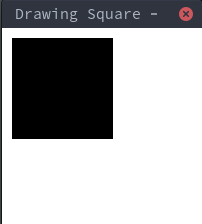
\includegraphics[width=0.3\linewidth]{./img/ensyuu1.png}
\end{center}
\section{演習2}
\label{sec:org5ce3664}
 上記のプログラムを入力して実行せよ。また、そのプログラムを改造して、 fill(255, 0, 0) を使って、図1のように赤白の市松模様が表示されるプログラムを作れ。\\
\subsection{上記のプログラムを入力して実行せよ。}
\label{sec:org0ccfd83}
\begin{minted}[frame=lines,linenos=true,obeytabs,tabsize=4]{clojure}
(defn ensyuu-2-1 []
  (q/defsketch draw-squares
    :title "Draw Squares"
    :setup (fn []
             (q/frame-rate 30)
             (q/color-mode :rgb)
             {:black 0
              :white 255})
    :size [200 200]
    :draw (fn [state]
                    (loop [i 0] ;; loop 関数:初期値は i = 0
                      (when (> 10 i) ;; もし 10 > i であるならば以下を実行する (*)
                        (do (if (zero? (mod i 2)) ;; もし i が 2 で ...
                              (q/fill 0) ;; 割り切れるならば、黒で塗りつぶすモードにする
                              (q/fill 255)) 
                              ;; 割り切れないならば、白で塗りつぶすモードにする
                            (q/rect (* i 10) (* i 10) 10 10) 
                            ;; (現在のモードで)四角形を表示する
                            (recur (inc i)))))) ;; i を 1 足してもう一度 (*) へ行く
                       ;; i <= 10 になれば recur が実行されず loop を抜ける
    :middleware [m/fun-mode m/pause-on-error]))
\end{minted}
 以上のプログラムを実行することで以下の結果を得る。\\
\begin{center}
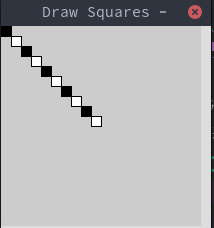
\includegraphics[width=0.3\linewidth]{./img/ensyuu2.png}
\end{center}
\subsection{赤白の市松模様が表示されるプログラムを作れ。}
\label{sec:org69f4533}
\begin{minted}[frame=lines,linenos=true,obeytabs,tabsize=4]{clojure}
(defn ensyuu-2-2 []
  (q/defsketch draw-ichimatsu
    :title "Draw Ichimatsu"
    :setup (fn []
             (q/frame-rate 30)
             (q/color-mode :rgb)
             {})
    :size [200 200]
    :draw (fn [state]
            (loop [i 0]
              (when (< i (* 10 10)) ;; i < 10 * 10 ならば以下を実行する
                (do
                 ;; i を 10 で割った 商と余りの和 が 2 で ...
                  (if (zero? (mod (+ (quot i 10) 
                                     (mod i 10)) 2))
                    (q/fill 255 0 0) ;; 割り切れるならば、fill(255, 0, 0)
                    (q/fill 255 255 255)) ;; 割り切れないならば fill(255, 255, 255)
                  (q/rect (* 20 (quot i 10)) ;; 四角形を描画する
                          (* 20 (mod i 10))
                          20
                          20)
                  (recur (inc i)))))
            )
    :middleware [m/fun-mode m/pause-on-error]))   
\end{minted}
 以上のプログラムを実行することで以下の結果を得る。\\
\begin{center}
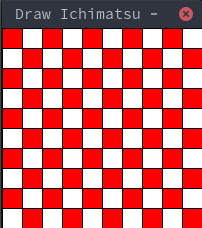
\includegraphics[width=0.3\linewidth]{./img/ensyuu3.png}
\end{center}
\section{演習3}
\label{sec:org5d861e1}
 マウスボタンを改造して、マウスボタンを押しているときだけ、四角形の枠が赤くなるようにせよ。なお、枠の色を帰るには stroke() を使う。\\
\begin{minted}[frame=lines,linenos=true,obeytabs,tabsize=4]{clojure}
(defn ensyuu-3 []
  (q/defsketch mouse-press-event
    :title "Mouse Event"
    :setup (fn []
             (q/frame-rate 30)
             (q/color-mode :rgb)
             {})
    :size [200 200]
    :mouse-pressed (fn [state event] ;; マウスボタンが押されたときに呼び出される関数
                     (q/stroke 255 0 0)) ;; 枠の色を変える
    :mouse-released (fn [state event] ;; マウスボタンが離されたときに呼び出される関数
                     (q/stroke 0 0 0)) ;; 枠の色を変える
    :draw (fn [state]
           (q/fill 255 255 255)
           (q/rect 20 20 60 60))
    :middleware [m/fun-mode m/pause-on-error]))
\end{minted}
 以上のプログラムを実行することで以下の結果を得る。\\
\begin{figure}[htbp]
\centering
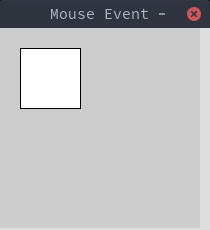
\includegraphics[width=0.3\linewidth]{./img/ensyuu3-2.png}
\caption{マウスボタンが離れているとき}
\end{figure}

\begin{figure}[htbp]
\centering
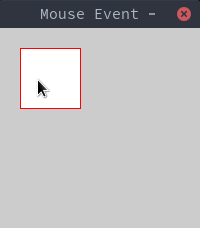
\includegraphics[width=0.3\linewidth]{./img/ensyuu3-1.png}
\caption{マウスが押されているとき}
\end{figure}

\subsection{イベント処理について}
\label{sec:org4a9d419}
イベント処理は手続き型言語のようにソースコードの頭から順番に実行される考え方とは異なり、例えば ``マウスが押されたとき'' といったイベントによって処理されることを示している。演習3 でいうならば、 Quil に登録されている mouse-pressed (Processing では mousePressed)に関数(Processing では手続き) を登録することで、マウスが押されたタイミングでこのイベント処理が行われる。\\

\section{演習4}
\label{sec:org85b5f83}
 r, g, b 以外の適当なキーを押すことで、表示される図形の形や大きさが変えられるようにせよ。\\
\begin{minted}[frame=lines,linenos=true,obeytabs,tabsize=4]{clojure}
(defn ensyuu-4 []
  (let [func (atom 0)] ;; ローカル変数の宣言(描画する図形を変化させるために使用)
   (q/defsketch key-press-event
     :title "Key Press Event"
     :setup (fn []
              (q/frame-rate 30)
              (q/color-mode :rgb)
              (q/background 100)
              {})
     :size [300 300]
     :mouse-pressed (fn [state event] ;; マウスボタンが押されたたら
                      (q/stroke 255 0 0)) ;; 線の色を変える
     :mouse-released (fn [state event] ;; マウスボタンが離されたら
                       (q/stroke 0 0 0)) ;; 線の色を変える
     :key-pressed (fn [_ {:keys [key key-code]}] ;; キーが押されたら
                    (case key ;; 以下の中から該当する物に対応した関数を実行する
                      :r (q/fill 255 0 0) ;; 赤くする
                      :g (q/fill 0 255 0) ;; 緑にする
                      :b (q/fill 0 0 255) ;; 青にする
                      :c (reset! func (if (zero? @func) 1 0))))
                      ;; 描画する図形を丸<=>四角にトグルする
     :draw (fn [state]
             (let [r (if (q/mouse-pressed?) 20 10)]
                ;; マウスが押されているならば r に 20 押されていないなら 10 を入れる。
               (if (zero? @func) ;; 描くべき図形をローカル変数 func から調べる
                 (q/ellipse (q/mouse-x) (q/mouse-y) r r) ;; 0 なら 丸を描く
                 (q/rect (q/mouse-x) (q/mouse-y) r r)))) ;; 1 なら 四角を描く
     :middleware [m/fun-mode m/pause-on-error])))
\end{minted}
 以上のプログラムを実行することで以下の結果を得る。\\
\begin{center}
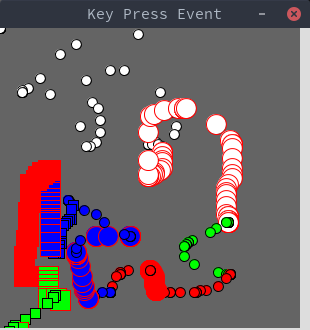
\includegraphics[width=0.3\linewidth]{./img/ensyuu4.png}
\end{center}

\section{演習5}
\label{sec:orgb293517}
 軌跡が正方形になるように動くように改造せよ。\\
\begin{minted}[frame=lines,linenos=true,obeytabs,tabsize=4]{clojure}
(defn ensyuu-5 []
  (let [func (atom 0)]
    (q/defsketch sikaku
      :title "sikaku"
      :setup (fn []
               (q/frame-rate 30)
               (q/color-mode :rgb)
               (q/background 100)
               {:len 0}) ;; len を現在の描いた長さを持つ変数として宣言
                         ;; 上の func 変数の位置に宣言しても同様の使い方が出来るが、
                         ;; Processing の update 関数を用いるためこちらに宣言した
      :size [300 300]
      :update (fn [state] ;; Processing にある update 関数
                {:len (if (== (:len state) 800) 0 (inc (:len state)))}) 
                ;; len を 増加させ、 800 を超えたらリセットする
      :draw (fn [state]
              (let [len (:len state)]
                (cond
                  (and (< 0 len) (<= len 200)) ;; 0 より大きく 200 以下なら
                  (q/ellipse (+ 50 len) 50 10 10) ;; 右に進め
                  (and (< 200 len) (<= len 400)) ;; 200 より大きく 400 以下なら
                  (q/ellipse 250 (- len 150) 10 10) ;; 下に進め
                  (and (< 400 len) (<= len 600)) ;; 400 より大きく 600 以下なら
                  (q/ellipse (- 250 (- len 400)) 250 10 10) ;; 左に進め
                  (and (< 600 len) (<= len 800)) ;; 600 より大きく 800 以下なら
                  (q/ellipse 50 (- 250 (- len 600)) 10 10) ;; 上に進め
                  )
                ))
      :middleware [m/fun-mode m/pause-on-error])))
\end{minted}
 以上のプログラムを実行することで以下の結果を得る。\\
\begin{center}
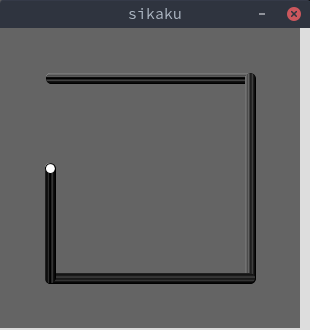
\includegraphics[width=0.3\linewidth]{./img/ensyuu5.png}
\end{center}

\section{演習6}
\label{sec:orgeddd7dd}
 メニューを使って、日付けを入力できるプログラムを作れ。つまり、月、日、曜日の3つをメニューで入力できるようにせよ。\\
\begin{minted}[frame=lines,linenos=true,obeytabs,tabsize=4]{clojure}
(defn ensyuu-6 []
  (q/defsketch input-date
    :title "Input Date"
    :size [400 150]
    :setup (fn []
             (let [cp (ControlP5. (quil.applet/current-applet))
                      ;; cp = new ControlP5(this) の意味
                      ;; Quil では this へ quil.applet/current-applet でアクセスする
                   dl1 (.addScrollableList cp "Month")
                      ;; cp.addScrollableList("Month") の意味
                      ;; Clojure の構文では (関数 インスタンス 引数) の順に書く
                   dl2 (.addScrollableList cp "Date")
                   dl3 (.addScrollableList cp "Week")
                   myfunc (fn [dl]
                            (-> dl ;; dl に対して
                                (.setSize 100 120) 
                                ;; (.setSize [dl] 100 120) するという意味
                                ;; 関数のすぐ隣に dl が挿入されている
                                (.setBarHeight 20)
                                (.setItemHeight 20)
                                ;; つまり、 dl.setSize(100, 120)
                                ;;           .setBarHeight(20)
                                ;;           .setItemHeight(20)
                                ))
                   _ (-> dl1
                         (.setPosition 50 10)
                         (myfunc)
                         (.addItems
                          '("Jan." "Feb." "Mar." "Apr." "May" "Jun." 
                            "Jul." "Aug." "Sep." "Oct." "Nov." "Dec.")
                            ;; リストを意味している
                            ))
                   _ (-> dl2
                         (.setPosition 150 10)
                         (myfunc)
                         (.addItems
                          (map str (take 31 (iterate inc 1))
                          ;; (iterate inc 1) 1 がスタートで、1を加算していく数列
                          ;; => 1 2 3 4 ...
                          ;; (take 31 ...) 先頭から 31 個要素を取り出す
                          ;; (map str ...) それぞれについて文字列型に変換する
                          )))
                   _ (-> dl3
                         (.setPosition 250 10)
                         (myfunc)
                         (.addItems
                          '("Mon." "Tue." "Wed." "Thu."
                            "Fri." "Sat." "Sun.")))]
               (q/frame-rate 30)
               (q/color-mode :rgb)))
    :draw (fn [] (q/background 100))
    :middleware [m/pause-on-error]))
\end{minted}
 以上のプログラムを実行することで以下の結果を得る。\\

\begin{center}
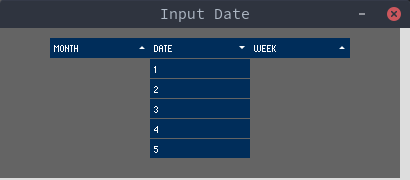
\includegraphics[width=0.3\linewidth]{./img/ensyuu6-1.png}
\end{center}

\begin{center}
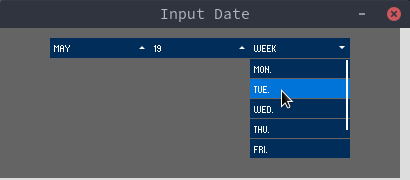
\includegraphics[width=0.3\linewidth]{./img/ensyuu6-2.png}
\end{center}

\subsection{Processing+controlP5 におけるGUI部品のレイアウト記述方法とイベント処理の記述方法}
\label{sec:org40bc3e0}
 ControlP5では GUI 部品のレイアウトは生成したインスタンスについて関数を適用していくことでレイアウトを設定する。またイベント処理は、命名した名前をつけた関数がイベント処理を行う関数になる。例えば ``b1'' というボタンを作れば、``b1''という関数がそのボタンを押した際のイベント処理を記述した関数になる。\\
\end{document}
